%%%%%%%%%%%%%%%%%%%%%%%%%%%%%%%%%%%%%%%%%%%%%%%%%%%%%%%%%%%%%%%%%%%%%%%%%%%%%%%%
%                            Document Information                              %
% ---------------------------------------------------------------------------- %
% Document Title: Identities with Vertex-, Edge-, and Mixed-metric Dimensions  %
% Created by: Lucija Tekavec & Martin Čadež                                    %
% Date Created: 2024/11/05                                                     %
% Version: 1.0                                                                 %
% ---------------------------------------------------------------------------- %
% Purpose: This LaTeX document is configured for academic report writing.      %
% ---------------------------------------------------------------------------- %
% Last Updated: 2024/11/14                                                     %
%%%%%%%%%%%%%%%%%%%%%%%%%%%%%%%%%%%%%%%%%%%%%%%%%%%%%%%%%%%%%%%%%%%%%%%%%%%%%%%%

% TODO List:
% - Add Definition and ILP for Edge Metric and Mixed Metric
% - Add Example for Edge Metric and Mixed Metric

%%%%%%%%%%%%%%%%%%%%%%%%%%%%%%%%%%%%%%%%%%%%%%%%%%%%%%%%%%%%%%%%%%%%%%%%%%%%%%%%
%                         Preamble Setup for Document                          %
%%%%%%%%%%%%%%%%%%%%%%%%%%%%%%%%%%%%%%%%%%%%%%%%%%%%%%%%%%%%%%%%%%%%%%%%%%%%%%%%

% --- General Document Settings ------------------------------------------------
\documentclass[12pt]{amsart}

% --- Page Layout and Geometry -------------------------------------------------
\usepackage[letterpaper, margin=1in]{geometry}

% --- Font and Microtype Settings ----------------------------------------------
\usepackage{microtype}

% --- Mathematical Symbols and Fonts -------------------------------------------
\usepackage{amsmath}
\usepackage{amssymb}
\usepackage{amsthm}
\usepackage{amsfonts}
\usepackage{mathrsfs}
\usepackage{bm}
\usepackage{mathtools}

% --- Tables and Arrays --------------------------------------------------------
\usepackage{booktabs}
\usepackage{makecell}
\usepackage{tabularray}

% --- Graphics and Color -------------------------------------------------------
\usepackage{graphicx}
\usepackage{xcolor}
\usepackage{pgfplots}

% --- Section and Formatting Control -------------------------------------------
\usepackage{titlesec}
\usepackage{setspace}
\usepackage{parskip}
\usepackage{ragged2e}

% --- Text Formatting ----------------------------------------------------------
\usepackage[normalem]{ulem}
\usepackage{mdframed}
\usepackage{hyphenat}

% --- Lists and Enumerations ---------------------------------------------------
\usepackage{enumitem}

% --- Hyperlinks and URLs ------------------------------------------------------
\usepackage{url}
\usepackage{hyperref}

% --- Miscellaneous ------------------------------------------------------------
\usepackage{circledsteps}
\usepackage{fancyhdr}

% \usepackage{tikz}
% \usetikzlibrary{patterns}
% \usetikzlibrary{backgrounds}

%%%%%%%%%%%%%%%%%%%%%%%%%%%%%%%%%%%%%%%%%%%%%%%%%%%%%%%%%%%%%%%%%%%%%%%%%%%%%%%%
%                       Custom Commands and Environments                       %
%%%%%%%%%%%%%%%%%%%%%%%%%%%%%%%%%%%%%%%%%%%%%%%%%%%%%%%%%%%%%%%%%%%%%%%%%%%%%%%%

% --- Theorem Environments Formatting ------------------------------------------
\theoremstyle{plain}
\newtheorem{theorem}{Theorem}[section]
\newtheorem*{proposition}{Proposition}
\newtheorem*{definition}{Definition}

% --- Color Definitions --------------------------------------------------------
\definecolor{color_blue_1}{HTML}{3276e3}
\definecolor{color_blue_2}{HTML}{b5dcff}
\definecolor{color_1_pink}{HTML}{ed4ac4}

% --- Table of Contents Depth --------------------------------------------------
\setcounter{tocdepth}{1}

% --- Page Layout and Geometry -------------------------------------------------
\geometry{
  top=2.2cm,
  headheight=0mm,
  headsep=0mm,
}
\pagestyle{fancy}
\fancyhf{}

% --- Header and Footer Rules --------------------------------------------------
\renewcommand{\headrulewidth}{0pt}
\renewcommand{\footrulewidth}{0pt}
\setlength{\footskip}{44pt}
\fancyfoot[C]{\thepage}

% --- Section Formatting -------------------------------------------------------
\titleformat{\section}
{\Large\bfseries}
{}
{0pt}
{}

% --- Spacing Definitions ------------------------------------------------------
\pgfplotsset{compat=newest}

%%%%%%%%%%%%%%%%%%%%%%%%%%%%%%%%%%%%%%%%%%%%%%%%%%%%%%%%%%%%%%%%%%%%%%%%%%%%%%%%
%                            End of Preamble Setup                             %
%%%%%%%%%%%%%%%%%%%%%%%%%%%%%%%%%%%%%%%%%%%%%%%%%%%%%%%%%%%%%%%%%%%%%%%%%%%%%%%%

\begin{document}

\begin{titlepage}
  \centering
  \Large \textsc{University of Ljubljana} \\[0.3cm]
  \textsc{\large Faculty of Mathematics and Physics}\\[2.5cm]

  \vspace{2.5cm}

  \scalebox{1.2}{\Large Investigating Graph Metric Identities}\\[0.3cm]
  \large School Project 2024/25 \\[1.8cm]
  \scalebox{3.5}{\textbf{REPORT}}\\[0.5cm]

  \vspace{0.3cm}

  \Large{Lucija Tekavec \& Martin Čadež} \\[0.2cm]

  \vspace{1.2cm}

  \begin{figure}[h!]
    \includegraphics[width=0.38\textwidth, height=0.28\textheight]{../figures/petersen_graph.png}
    \label{fig:petersen_graph}
  \end{figure}
  \vspace{0.3cm}

  \large{Mentors: \\ doc. dr. Janoš Vidali, \\ prof. dr. Riste Škrekovski} \\[0.2cm]
  \vfill

\end{titlepage}

\newpage

\section{\huge Introduction}
This report presents the findings of our investigation into the \textit{metric dimensions} of graphs, specifically focusing on the two relationships among the metric dimension, the edge metric dimension, and the mixed metric dimension of a graph. Our objective is the following:

\vspace{0.2cm}

\begin{mdframed}[backgroundcolor=color_blue_1!10, linecolor=color_blue_2, linewidth=2pt, roundcorner=10pt, innertopmargin=10pt, innerbottommargin=10pt, skipabove=5pt, skipbelow=5pt]
  \textbf{Problem Statement:} Let \textbf{$G$} $ \in \mathcal{G}(V, E)$ be a connected graph with $\textit{\textbf{dim(G)}}$, $\textit{\textbf{edim(G)}}$, and $\textit{\textbf{mdim(G)}}$ representing the metric dimension, edge metric dimension, and mixed metric dimension of $G$, respectively. Objective is to find graphs $G \in \mathcal{G}$ such that one of the following relationships holds:
  \begin{enumerate}
      \centering
    \item $\textit{\text{dim(G)}} = \textit{\text{edim(G)}} + \textit{\text{mdim(G)}}$
    \item $\textit{\text{mdim(G)}} = \textit{\text{dim(G)}} + \textit{\text{edim(G)}}$
  \end{enumerate}
\end{mdframed}

\vspace{0.2cm}

Before we delve deeper, we need to clarify some of the key concepts and ideas that will be foundational to our problem. Let's define some key terms.

\vspace{0.2cm}

\section{Prelimitary Definitions}

Since we need to understand the concept of \textit{resolving sets} for definition of metric dimension, we will first explain when vertex is resolved by a set of vertices. We say that a vertex $s$ \textit{resolves} a pair of vertices $v_1$ and $v_2$ if the shortest distance between $v_1$ and $s$ is different from the shortest distance between $v_1$ and $s$, i.e. $d(v_1, s) \neq d(v_2, s)$. Let's examine one example:

\vspace{-0.2cm}

\begin{figure}[h!]
  \centering
  \begin{minipage}{0.42\textwidth}
    \centering
    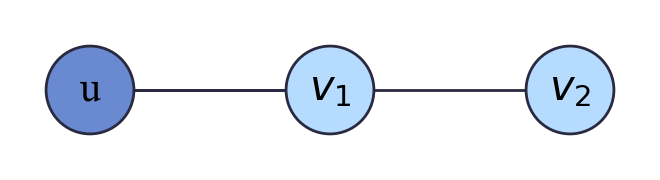
\includegraphics[width=\textwidth]{../figures/res_vertex_fig1.png}
    \label{fig:res_vertex_fig1}
  \end{minipage}
  \hspace{0.08\textwidth}
  \begin{minipage}{0.42\textwidth}
    \centering
    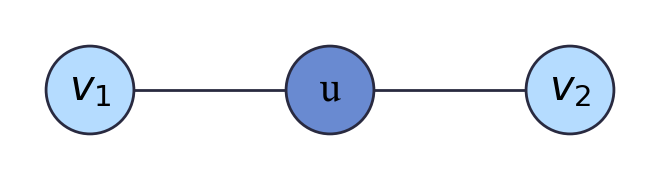
\includegraphics[width=\textwidth]{../figures/res_vertex_fig2.png}
    \label{fig:res_vertex_fig2}
  \end{minipage}
\end{figure}

\vspace{-0.5cm}

In the left graph, vertex $s$ resolves vertices $v_1$ and $v_2$, because $d(v_1, s) = 1$ and $d(v_2, s) = 2$, while in the right graph, vertex $s$ does not resolve $v_1$ and $v_2$ since $d(v_1, s) = d(v_2, s) = 1$.

\vspace{-0.2cm}

\begin{definition} \textbf{(Resolving Set)} \\[1pt]
  Set $S \subseteq V(G)$ is a \textit{resolving set} of a graph $G$ if for every pair of distinct vertices $u, v \in V(G)$, there exists a vertex $s \in S$ such that $d(u, s) \neq d(v, s)$.
\end{definition}

\vspace{-0.2cm}

For better understanding of resolving sets, it is essential to understand how vertices can be uniquely distinguished based on their distances to specific subsets of the graph.

\vspace{-0.2cm}

\begin{definition} \textbf{(Metric Representation)} \\[1pt]
  Let $G \in \mathcal{G}(V, E)$ and $W \subseteq V(G)$ be an ordered set. \textit{Metric representation} of $G$ is a function $r: V(G) \rightarrow \mathbb{R}^{|W|}$ defined as $r(v \mid W) = (d(v, w_1), d(v, w_2), \ldots, d(v, w_{|W|}))$ for all $v \in V(G)$.
\end{definition}

\vspace{-0.2cm}

Set $W \subseteq V(G)$ is also called \textit{set of representatives} of $G$ and it has important connection to resolving sets. But first, let's look into metric representations for two graphs from above. If we chose $W = \{s\}$, then metric representation of the left graph would be $r(v_1 \mid W) = (1)$ and $r(v_2 \mid W) = (2)$, while for the right graph, $r(v_1 \mid W) = (1)$ and $r(v_2 \mid W) = (1)$. This leads us to the following proposition:

\newpage

\begin{proposition} \textbf{(Resolving Set Criterion)} \\
  Set of representatives $W \subseteq V(G)$ is a resolving set of $G$ if and only if the distinct vertices $u, v \in V(G)$ have distinct metric representation, i.e. $\forall u,v \in V, u \neq v : r(u \mid W) \neq r(v \mid W)$.
\end{proposition}

\vspace{-0.2cm}

Let's look into another example for better understanding. Consider the following graphs:

\vspace{-0.4cm}

\begin{figure}[h!]
  \centering
  \begin{minipage}{0.42\textwidth}
    \centering
    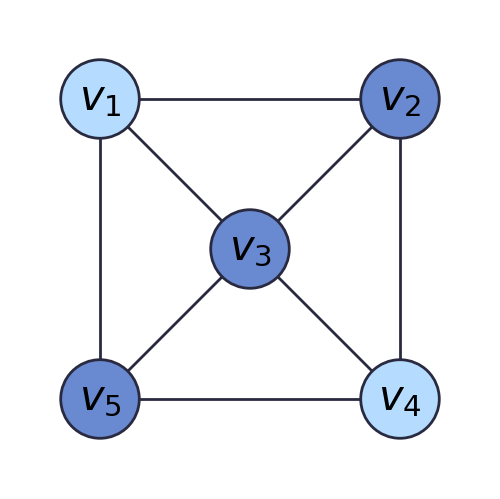
\includegraphics[width=\textwidth]{../figures/res_set_fig1.png}
    \label{fig:res_set_fig1}
  \end{minipage}
  \hspace{0.08\textwidth}
  \begin{minipage}{0.42\textwidth}
    \centering
    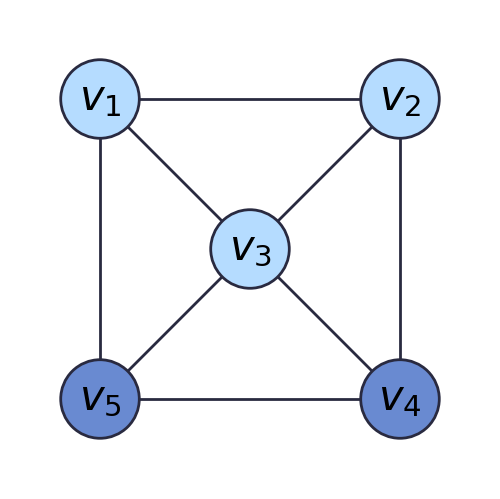
\includegraphics[width=\textwidth]{../figures/res_set_fig2.png}
    \label{fig:res_set_fig2}
  \end{minipage}
\end{figure}
\vspace{-1cm}
\begin{minipage}[t]{0.45\textwidth}
  In the left graph, set of representatives is $ W_1 = \{ v_2, v_3, v_5 \} $ and the folowing metric representation are: \\[1pt]
  \vspace{-0.4cm}
  \begin{align*}
    r(v_1 \mid W_1) &= (1, 1, 1) \\
    r(v_2 \mid W_1) &= (0, 1, 2) \\
    r(v_3 \mid W_1) &= (1, 0, 1) \\
    r(v_4 \mid W_1) &= (1, 1, 1) \\
    r(v_5 \mid W_1) &= (2, 1, 0)
  \end{align*}
\end{minipage}
\hfill
\begin{minipage}[t]{0.45\textwidth}
  While on the right graph, $W_2 = \{ v_4, v_5 \} $ and this selection corresponds to the following metric representations: \\[1pt]
  \vspace{-0.4cm}
  \begin{align*}
    r(v_1 \mid W_2) &= (2, 1) \\
    r(v_2 \mid W_2) &= (1, 2) \\
    r(v_3 \mid W_2) &= (1, 1) \\
    r(v_4 \mid W_2) &= (0, 1) \\
    r(v_5 \mid W_2) &= (1, 0)
  \end{align*}
\end{minipage}

Set $W_1$ is not the resolving set, because $r(v_1 \mid W_1) = r(v_4 \mid W_1) $, while on the onther hand $W_2$ is resolving set since every metric representation is distinct. Now, with better understanding of resolving sets, we are prepared to define \textit{graph metric dimension}, notated with $ dim(G)$.

\vspace{-0.2cm}

\begin{definition} \textbf{(Metric Basis)} \\
  \textit{Metric basis} of connected graph $G$ is a smallest resolving set of $G$.
\end{definition}

\vspace{-0.4cm}

\begin{definition} \textbf{(Metric Dimension)} \\
  \textit{Metric dimension} of a connected graph $G$ is the minimum cardinality of a resolving set of $G$.
\end{definition}

\vspace{-0.3cm}

In other words, the metric dimension seeks the smallest subset of vertices that can uniquely identify all other vertices in the graph based on their distances.

It is crucial to highlight that determining the metric dimension is an NP-hard problem, indicating that no polynomial-time solution is known for solving this problem in general cases. Consequently, finding an optimal resolving set requires the use of heuristic or approximation methods in practical applications.

\vspace{-0.2cm}

\begin{proposition} \textbf{(Metric Dimension's Bounds)} \\
  Let $ G(V, E) $ be a connected graph with $|V| = n $ vertices. The metric dimension of $G$, denoted by $dim(G)$  is bounded by: $ 1 \leq dim(G) \leq n-1 $.
\end{proposition}

\newpage

As discussed above, determining metric dimension of a graph poses significant computational challenges, but for some graphs, analytical methods have been established \cite{metric_dim_ALGO}. Those are:

\begin{itemize}
  \item Complete Graphs with $n$ vertecies : $ dim (K_n) = n - 1 $
  \item Path Graphs with $n$ vertecies : $ dim (P_n) = 1 $
  \item Star Graphs with $n$ vertecies : $ dim (S_n) = n - 2 $
  \item Cycle Graphs with $n$ vertecies : $ dim (C_n) = 2 $
  \item Bipartite Graphs between two sets of vertecies $t$ and $s$ : $ dim(K_{s,t}) = s + t - 2, t \geq 1$
\end{itemize}

What about in general? How do we determine metric dimension? Let us explore computation of the K-metric dimension in greater detail \cite{metric_dim_ILP}.

\vspace{0.1cm}

\begin{mdframed}[backgroundcolor=color_blue_1!10, linecolor=color_blue_2, linewidth=2pt, roundcorner=10pt, innertopmargin=10pt, innerbottommargin=10pt, skipabove=5pt, skipbelow=5pt]
  \textbf{Integer Linear Programe for K-metric dimension:} \\[3pt]
  Let $ G \in \mathcal{G}(V,E)$ be a connected graph with vertex set $ V(G) = \{v_1, v_2, v_3, v_4, v_5 \} $ and $D_G$ a distance matrix defined as $ D_G = [d_{ij}]_{i,j = 1}^{n}$, where $d_{ij} = d_G(v_i, v_j)$. Note : $ |V(G)| = n $.

  objective : $ \textit{min} \left( \, \sum\limits_{\, h=1}^{n} x_h \right)$ \\
  subject to :
  \begin{enumerate}

    \item \quad
      $
      \forall i \, \forall j , 1 \leq i < j \leq n \, : \, \sum\limits_{h=1}^{n} \delta(d_{ih}, d_{jh}) \, x_h \, \geq \, K
      $
    \item \quad
      $
      \forall h \in \{1, \ldots, n \} \, : \, x_h \in \{0,1 \}
      $
  \end{enumerate}
  where :
  \begin{enumerate}
    \item \quad
      $
      \delta(d_{ij}, d_{i'j'}) =
      \begin{cases}
        \, 1 & \! ; \, \, \, d_{ij} \neq d_{i'j'} \\
        \, 0 & \! ; \, \, \, d_{ij} = d_{i'j'}
      \end{cases}
      $
    \item \quad
      $
      x_h =
      \begin{cases}
        1 & \! ; \, \, \, v_h \, \, \text{is included in metric basis} \\
        0 & \! ; \, \, \, otherwise
      \end{cases}
      $
  \end{enumerate}

  \vspace{0.2cm}

  If a given ILP is feasible for chosen treshold $K$ and $(x_1^*, x_2^*, \ldots, x_n^* )$ is optimal solution, then the set $ W = \{v_i \mid x_i^* = 1\} $ forms a $K$-metric basis of $G$. So $|W| = dim^{(K)}(G)$.
\end{mdframed}

\vspace{0.1cm}

Let's give a short explanation. Since the primary goal is to identify the smallest possible subset of vertices that can uniquely distinguish all other vertices in the graph, we aim to minimize the number of selected vertices, represented by $ x_k $. In conjunction with this, the $ \delta $ - function serves as a binary comparison operator that determines whether a given vertex can resolve other vertices. Essentially, it checks whether a given vertex is part of the resolving set, which allows us to distinguish vertices based on their distances. Important to mention is the fact that, point (1) gives us $ \binom{n}{2} $ constrains.

Since we need to generate distance matrix, examine every distance and identify the optimal subset of vertices, this task becomes computationally challenging. Although the resulting equations are relatively straightforward to formulate, the sheer volume of combinations makes the problem computationally intensive and time-consuming.

\newpage

Remember the first example from above, ILP for metric dimension of $ P_3 $ graph is equal to :

\begin{minipage}[t]{0.4\textwidth}
  Distance matrix for given graph is :
  \vspace{0.2cm}
  $$
  D_{P_3} =
  \begin{bmatrix*}
    0 & 1 & 2 \\
    1 & 0 & 1 \\
    2 & 1 & 0
  \end{bmatrix*}
  $$
  \vspace{0.4cm}
  $K = 1$.
\end{minipage}%
\begin{minipage}[t]{0.55\textwidth}
  \vspace{-0.3cm}
  $$
  \begin{aligned}
    & \text{minimize} \quad x_1 + x_2 + x_3 \\
    & \,\, \text{s.t.} \\
    & \quad x_1 + x_2 + x_3 \geq 1, \\
    & \quad x_1 + x_3 \geq 1, \\
    & \quad x_1 + x_2 + x_3 \geq 1, \\
    & \,\, x_1, x_2, x_3 \in \{0, 1\}
  \end{aligned}
  $$
\end{minipage}

So the optimal solution $\mathbf{x}^{*}$ is either $[1,0,0]^{C} $ or $ [0,0,1]^{C} $.

\newpage

\begin{definition} \textbf{(Edge Metric)} \\
  The \textit{edge metric} of a graph $G$ is a metric defined on the edge set $E(G)$, where the distance between two edges $e_1, e_2 \in E(G)$ is the number of common vertices between the two edges.
\end{definition}

\begin{definition} \textbf{(Mixed Graph Metric)} \\
  The \textit{mixed graph metric} of a graph $G$ is a metric defined on the vertex-edge set $V(G) \cup E(G)$, where the distance between a vertex $v \in V(G)$ and an edge $e \in E(G)$ is the number of common vertices between the vertex $v$ and the edge $e$.
\end{definition}

\newpage

\begin{thebibliography}{9}

  \bibitem{petersen}
  Petersen Graph. (2024). \textit{Petersen Graph}. Wikipedia. Available \href{https://en.wikipedia.org/wiki/Petersen_graph}{\textit{here}}.

  \bibitem{yt_video_1}
  Wrath of Math. (2020, April 13th). \textit{Resolving Sets and Metric Dimension of Graphs | Graph Theory} [Video]. YouTube. Available \href{https://www.youtube.com/watch?v=ESgQnbHTj7c}{\textit{here}}.

  \bibitem{metric_dim_ILP}
  Sandi Klavžar, Freydoon Rahbarnia, Mostafa Tavakoli. (2021,February 12th). \textit{Some binary products and integer linear programming for computing k-metric dimension of graphs}. arXiv:2101.10012v2 [math.CO]. Available
  \href{https://users.fmf.uni-lj.si/klavzar/preprints/2101.10012v2.pdf}{\textit{here}}

  \bibitem{metric_dim_ALGO}
  Muhammad, F., \& Susilowati, L. (2020). \textit{Algorithm and computer program to determine metric dimension of graph}. Journal of Physics: Conference Series, 1494, 012018. Available \href{https://iopscience.iop.org/article/10.1088/1742-6596/1494/1/012018}{\textit{here}}.

  \bibitem{edge_metric_dim_1}
  \href{https://users.fmf.uni-lj.si/klavzar/preprints/emd(Mar\%209\%202020)-submit.pdf}{\textit{here}}

\end{thebibliography}

\end{document}
